\documentclass[11pt,a4paper]{report}
\usepackage{pdfpages}
\usepackage{amssymb,amsmath}
\usepackage{enumitem}
\setlist{noitemsep,topsep=0pt,parsep=0pt,partopsep=0pt}

\usepackage{soul} % underlines
\setuldepth{aaaa}
\usepackage{framed}


%\usepackage[style=authoryear]{biblatex}
\usepackage[style=numeric,maxbibnames=19, maxcitenames=2,firstinits=true]{biblatex}
\addbibresource{biblio.bib}
\addbibresource{cogarch.bib}
\addbibresource{my-publications.bib}
\addbibresource{mutual-modelling.bib}

\usepackage{pdflscape}

\usepackage{fontspec}
\defaultfontfeatures{Ligatures=TeX,Scale=MatchLowercase}
\setmainfont[]{cantarell}

\usepackage{graphicx}
\graphicspath{{figs/}}
\usepackage{wrapfig}
\usepackage{hyperref}
\urlstyle{same}  % don't use monospace font for urls
\usepackage[margin=4pt]{subcaption}

\usepackage[a4paper,left=2cm,right=2cm,top=1.5cm,bottom=1.5cm]{geometry}
\usepackage{longtable,booktabs}

\usepackage{pgfgantt}
\usepackage{rotating}

\usepackage{tocloft}

\usepackage[compact]{titlesec}
\usepackage{blindtext, color}
\definecolor{gray75}{gray}{0.75}
\newcommand{\hsp}{\hspace{20pt}}
\titleformat{\chapter}[hang]{\LARGE\bfseries}{\textcolor{gray75}{|}\hsp}{0pt}{\LARGE\bfseries}
\titlespacing{\chapter}{0pt}{0pt}{0.5em}

%\titlespacing*{\section}
%{0pt}{5.5ex plus 1ex minus .2ex}{4.3ex plus .2ex}
%\titlespacing*{\subsection}
%{0pt}{5.5ex plus 1ex minus .2ex}{4.3ex plus .2ex}


\renewcommand{\thesubsubsection}{}

\usepackage{xspace}
\newcommand{\project}{WizUs\xspace}

\newcommand{\task}[2]{\vspace{0.5cm}\noindent\emph{Task T#1}: {\bf #2}\par}

\newcommand{\D}[3]{\emph{Deliverable D#1} (M#2): #3\\}

\newcommand{\TODO}[1]{{\color{red}\textbf{#1}}}
%\newcommand{\TODO}[1]{}

\newcommand{\severin}[1]{{\color{red}\textbf{Severin: #1}}}
\newcommand{\toseverin}[1]{{\color{red}\textbf{To Severin: #1}}}
%\newcommand{\eu}[1]{{\color{teal}\textbf{Guidelines EU ERC: #1}}}
\newcommand{\eu}[1]{}
\newcommand{\cellgrey}{\cellcolor[gray]{0.85}}

\setcounter{secnumdepth}{0} % prevent section numbering, but still add sections to ToC

\setlength\FrameSep{\fboxsep}

\title{\project -- Ethics \& Privacy}

\begin{document}

\begin{center}
    ERC Consolidator Grant 2020

    \vspace{2cm}

    \textbf{\LARGE \project -- Ethics \& Data Protection}

    \vspace{2cm}

\end{center}

\section{Ethics}

\subsection{National and European Legal and Ethical Requirements}

The University of the West of England (UWE) and Pr. Lemaignan,  as the Research
Lead for the \project project, will take responsibility for all ethical
considerations ensuring the project delivers the necessary standards to meet all
relevant national and European directives concerning Ethics. UWE will set the
standard for all stakeholders working with this project, by sharing best
practice to make ensure all project Partners follow the example delivered by
UWE; and comply where necessary with the Research Ethics Procedures as set down
in UWE Governance. 

UWE as a UK HEIs is bound by its funding organisation UK Research \& Innovation
(UKRI) to meet the requirements of the `Concordat to Support Research Integrity'
(Universities UK, 2012). This in turn binds all UK HEIs funded by UKRI to the
standards as set out by a number of funding organisations, including Research
Councils UK's `Integrity, clarity and good management: Research Councils UK
Policy and Code of Conduct on the Governance of Good Research' and the European
Science Foundation's `European Code of Conduct for Research Integrity'.  To
support this policy UWE set in place a \emph{Code of Good Research
Conduct}\footnote{\url{https://www1.uwe.ac.uk/research/researchgovernance/codeofgoodresearchconduct.aspx}}, from which
UWE's Ethical standards and procedures are stated and delivered.

\vspace{2em}

The partners involved in the project all have excellent standards for research
ethics. All partners have agreed to conform with those standards as set by the
UWE Research Ethics Process.  This process follows Directives on Research Ethics
as appropriate to the research field, which in turn bind UWE to the EU
Directives as set out in the Ethics Self-Assessment Guidance for Horizon
2020\footnote{\url{http://ec.europa.eu/research/participants/data/ref/h2020/grants_manual/hi/ethics/h2020_hi_ethics-self-assess_en.pdf}}.

The partners who will be supporting the engagement activities all have similar
Codes of Conducts for all employees to adhere to which details their roles and
responsibility to citizens, both in terms of conduct and their personal data.
Specifically:

\begin{itemize}
    \item The Bristol Science centre WeTheCurious has long participated in
        scientific research with the University of West and England and the
        University of Bristol, and have in place rigorous ethics and data
        management plans. Appendix 1 includes a recent example of Ethics
        application form for a large study that took place in the centre.
    \item the study at the Bristol Children's Hospital will be conducted in
        accordance to the strict UK National Health Service (NHS) ethics
        framework:
        \url{https://www.hra.nhs.uk/about-us/committees-and-services/res-and-recs/}
\end{itemize}



\subsection{Ethics Approval Process}

Pr. Séverin Lemaignan, as \project lead, will coordinate and manage all ethical
approval processes ensuring that all other Partners are in compliance. \textbf{Note that
an Ethics Approval Application can only be submitted to the UWE Research Ethics
Committee once a grant has been awarded}.

Appendices 1 and 2 include sample of ethics-related documents and plans produced
for previous studies with populations and environments similar to those of
\project. They evidence the experience of the project team in conducting safe
and responsible research.

\subsection{Potential Ethical Issues identified within \project}

The project will investigate how social robots can integrate into existing
social eco-systems (a museum, a paediatric ward, a school) over long period of
time (one year each), and what are the resulting social dynamics elicited by the
robot presence. As such (and as identified in the Ethics self-assessment form),
the \project project involves social robots, interacting in repeated ways and
over long period of time, with human end-users, including vulnerable children.

All efforts to ensure the health and safety of participants and researchers will
be undertaken: Risks to participants and the researchers will be considered in
any Risk Assessments taking for specific activities.  Full measures to ensure
safeguarding of children will be taken, following UWE Guidance on Research
involving
children\footnote{\url{http://www2.uwe.ac.uk/services/Marketing/research/pdf/Guidance-on-Research-with-Children.pdf}}.
Further information on Safeguarding is included in UWEs Ethical Guidance
documents\footnote{\url{http://www1.uwe.ac.uk/research/researchethics/guidance.aspx}}.
All researchers and staff involved in working with children or vulnerable adults
will have Disclosure and Barring Service (DBS) checks, and will have to attend the
training of Children Safeguarding offered by the university. In addition, they
will be under the supervision of trained staff members experienced at working
with vulnerable children.

Pr. Lemaignan has extensive experience in
conducting fieldwork with social robots and children (including vulnerable
children); Dr. Newbutt, who will support T5.1 (SEN schools study), has a
long-track record of conducting research with SEN schools; and Dr. Bowyer (T5.2,
Children's Hospital) is also experienced in conducting academic research within
the hospital, and familiar with the NHS ethics approval process.


For illustration purposes, Appendix 2 to this document include samples of
participant information sheet and informed consent forms used in a previous
study on VR, conducted by Dr. Newbutt with vulnerable children.

%The engagement methodologies detailed throughout the project also entail communication and
%dissemination where no data is collected. As such, only the engagement methodologies which
%collect data to be used within the research project have been detailed below, these are categorised
%by the various types of activity:
%
%\begin{enumerate}
%    \item {\bf Crowd-sourced social interaction pattern} -- this methodology,
%        essential to the museum study conducted in T1.2, involve voluntary
%        participation of accompanied children or adult visitors to control the robot.
%        All participants will receive written Participant Information Sheets and will
%sign Consent Forms before participation. Appropriate Participant Information Sheets and
%Consent Forms will be used to recruit people with limited understanding
%(children/vulnerable adults); for children under the age of 18 parental, guardian or class
%teacher consent will also be required; example formats are included at the end of this
%section (Appendix 2). Participants in face-to-face workshops will be given the option to
%withdraw from participation with due notice provision; if this happens, data files relating to
%the individual will be permanently deleted and records removed from the combined data
%profile (see Data Management Plan). The workshops will use semi-structured focus group
%formats to explore perceptions of the resulting scenarios and develop consensus outcomes.
%Meetings will be audio recorded and transcribed verbatim, then analysed with qualitative
%thematic analysis. All data will be kept in accordance with the Data Management Plan, then
%grouped to remain individually unidentifiable for reporting.
%
%\item {\bf Online surveys and games/app feedback} - Pre-workshop questionnaires will collect data on
%perceptions, attitudes and behaviours contributing to air quality. Data will also be collected
%on the dissemination and engagement processes (as detailed in dissemination plan), to
%evaluate their effectiveness. Post-workshop questionnaires will be distributed online and in
%person so the citizens can feedback on their involvement. Citizens contributing to the
%activities or other dissemination events and activities will also be invited to complete online
%questionnaires, or complete brief feedback measures (e.g. post-it notes) at events.
%Quantitative data on game/app usage will be collected through the game/app itself.
%
%\item{\bf Data} collected through online methods or in person written feedback at events will be
%flagged up with a written statement when the game/app/questionnaire is initiated; consent
%will be assumed if the participant continues. As the data collected via these methods is
%anonymous from initial participation, participants cannot withdraw their
%contribution.
%\end{enumerate}



\subsubsection{Additional measures}

In recognition of the complexity of the ethical questions raised by the project --
some of those actually raising new research questions --, the standard Ethics
assessment and approval process described above \textbf{will be complemented with a
dedicated research activity on ethics} (Task 1.1 of Workpackage 1) that will
contribute to establishing novel ethical guidelines for long-term deployments of
social robots. These guidelines will be modeled after the Ethics Guidelines for
Trustworthy AI, released in 2019 by the EU High-level Expert Group on Artificial
Intelligence.

Additionally, this work will be supported by a dedicated Ethics Advisory Board,
composed of 3 experts in ethics and social robotics and AI. While the exact
composition of the board is not final yet, it will include at least one member
from the EU High-Level Expert Group on Artificial Intelligence.


\section{Data management}

The University of the West of England is fully conversant and compliant with
the Data Protection Act of 2018 and specifically the \emph{General Data
Protection Regulation} (GDPR). UWE has created and implemented a \emph{Data
Protection Standard for Research and Researchers based at the
University}\footnote{\url{https://www1.uwe.ac.uk/research/researchgovernance/resourcesforresearchers/researchdatamanagement.aspx}},
linked to the UWE Data
Policy\footnote{\url{https://www2.uwe.ac.uk/services/Marketing/about-us/pdf/Policies/Data-Protection-Policy.pdf}},
with UWE's Data Protection Office\footnote{\url{dataprotection@uwe.ac.uk}} responsible for overseeing the
implementation of this policy, and monitoring the University's compliance with
data protection law.

The Data Protection Standard for Research provides  guidance on all stages of
the research process including project design, data protection generally,
retention and disposal. Each UWE Bristol research project is required to
demonstrate adherence to the Standard. In addition the Research Ethics
Application, Research Data Management Plan and Research Governance Record
reflects the researchers and their projects compliance. Specifically, UWE
researchers follow the University protocols and processes for working with
children and vulnerable adults and the corresponding data protection standards.

To ensure the appropriate collection of data, methods, and storage (servers) and
use in the project (models, publications, communications etc.), the strategy for
the collection and use of data across the project is documented in the \project
\emph{Data Management Plan} (DMP). This document uphold the principles of GDPR in
keeping with Regulation (EU) 2016/679 on the protection of natural persons with
regard to the processing of personal data and on the free movement of such
data\footnote{\url{https://ec.europa.eu/info/law/law-topic/data-protection/dataprotection-eu_en}}.
The \project \emph{Data Management Plan} will be published prior to the first
data collection (Task 1.2), and will be submitted as a part of the UWE Ethics
approval process. If necessary, the DMP will be revised prior to subsequent data
collection tasks, and in particular before the field experiments taking place in
WP5.

 
\eu{
If you have entered any ethics issues in the ethical issue table in the administrative proposal forms, you must:
    • submit an ethics self-assessment, which:
        ◦ describes how the proposal meets the national legal and ethical requirements of the country or countries where the tasks raising ethical issues are to be carried out;
        ◦ explains in detail how you intend to address the issues in the ethical issues table, in particular as regards:
        ◦ research objectives (e.g. study of vulnerable populations, dual use, etc.)
        ◦ research methodology (e.g. clinical trials, involvement of children and related consent procedures, protection of any data collected, etc.)
        ◦ the potential impact of the research (e.g. dual use issues, environmental damage, stigmatisation  of  particular  social  groups,  political  or  financial  retaliation, benefit-sharing,  malevolent use , etc.).
    • provide the documents that you need under national law(if you already have them), e.g.:
        ◦ an ethics committee opinion;
        ◦ the document notifying activities raising ethical issues or authorising such activities
 If these documents are not in English, you must also submit an English summary of them(containing, if available, the conclusions of the committee or authority concerned).
 If you plan to request these documents specifically for the project you are
 proposing, your request must contain an explicit reference to the project
 title.
}

\newpage
\section{Appendix 1: sample Ethics application and Consent forms for large scale
experiment at the WeTheCurious science centre}

Included hereafter are:

\begin{itemize}
    \item the full ethics application form for the SPHERE project, a
        longitudinal study that took place in 2018 at the WeTheCurious science
        centre. Similar to the requirements of the \project project, this study
        involved the participation of the visitors, both adults and children.
    \item Samples of consent forms (both for adults and minors) used for the
        SPHERE project.
\end{itemize}

Additional documents (like the Information sheets and questionnaires) are
available as well, were they required.

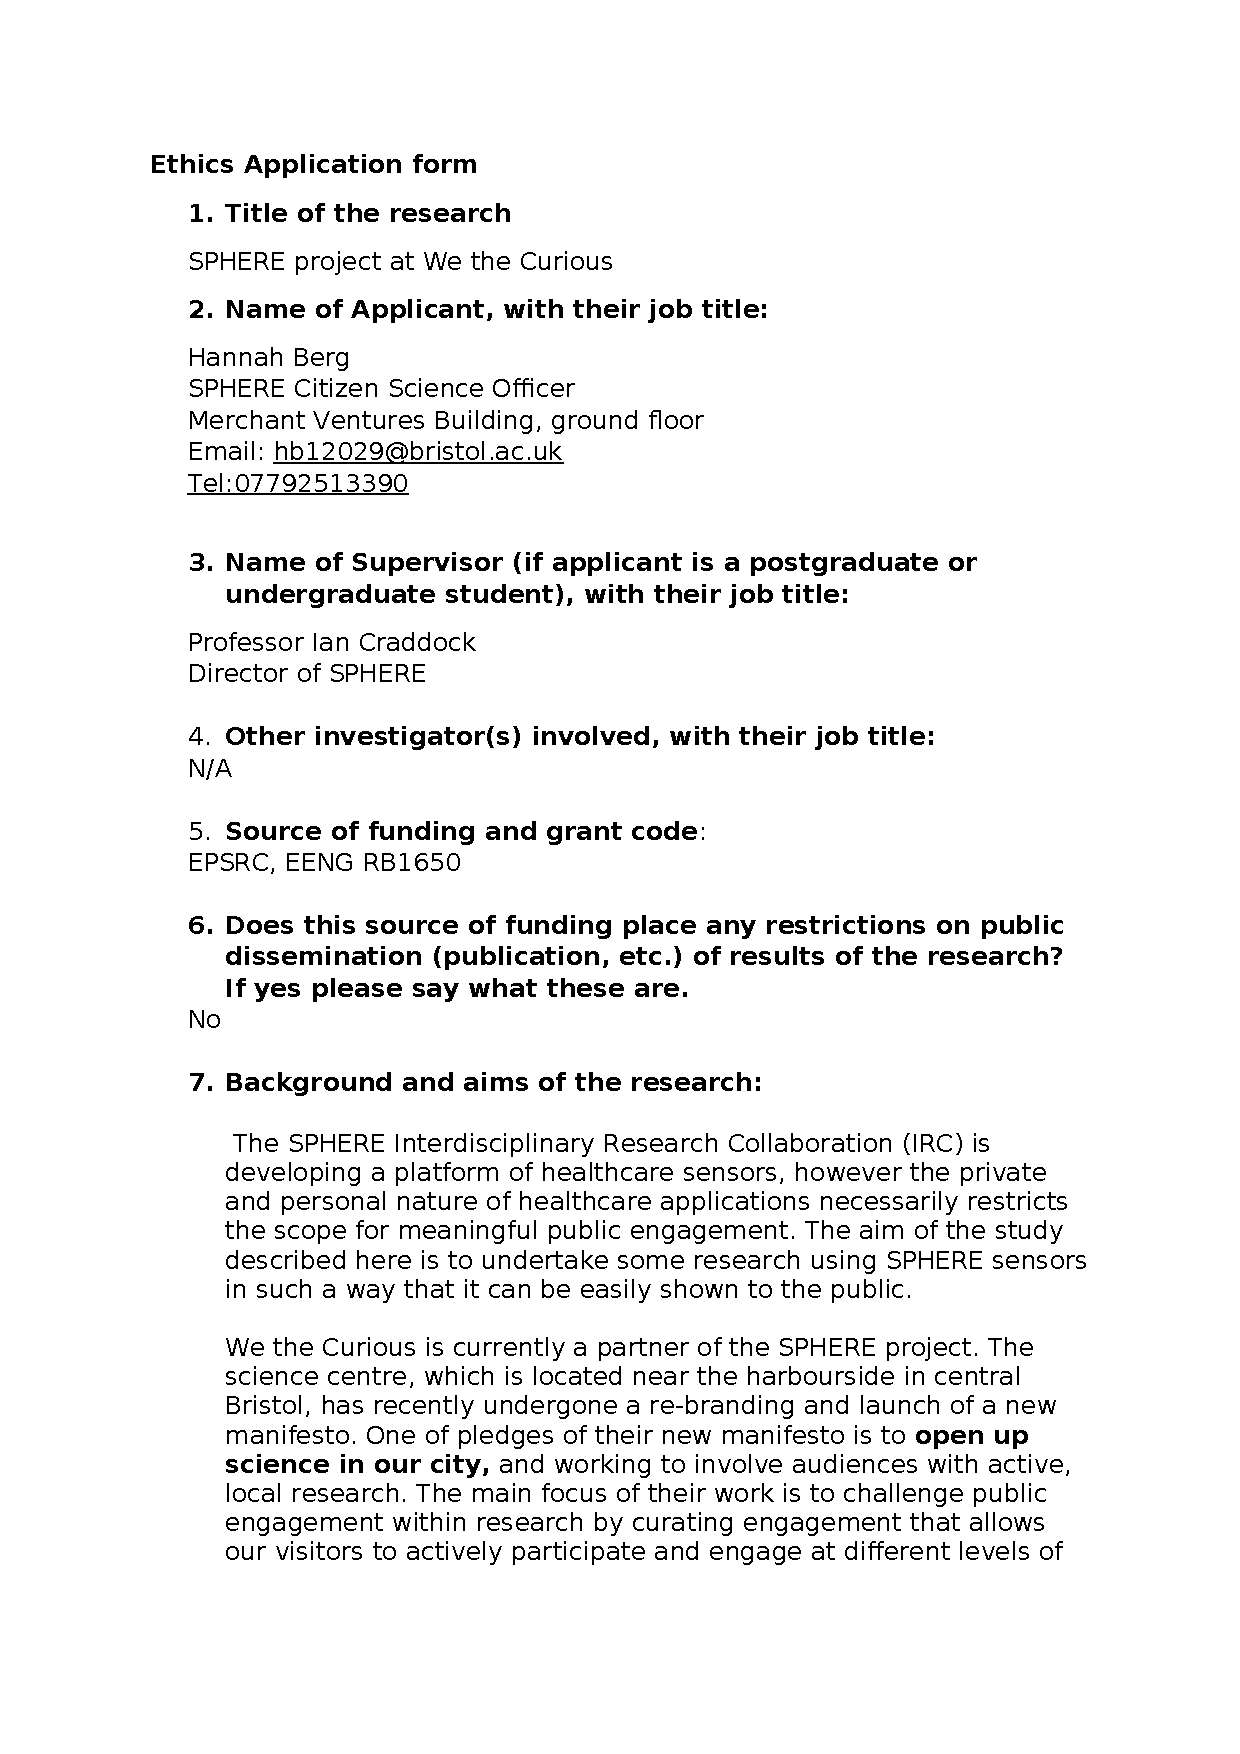
\includepdf[pages=-]{ethics/Ethics_Application_SPHERE.pdf}
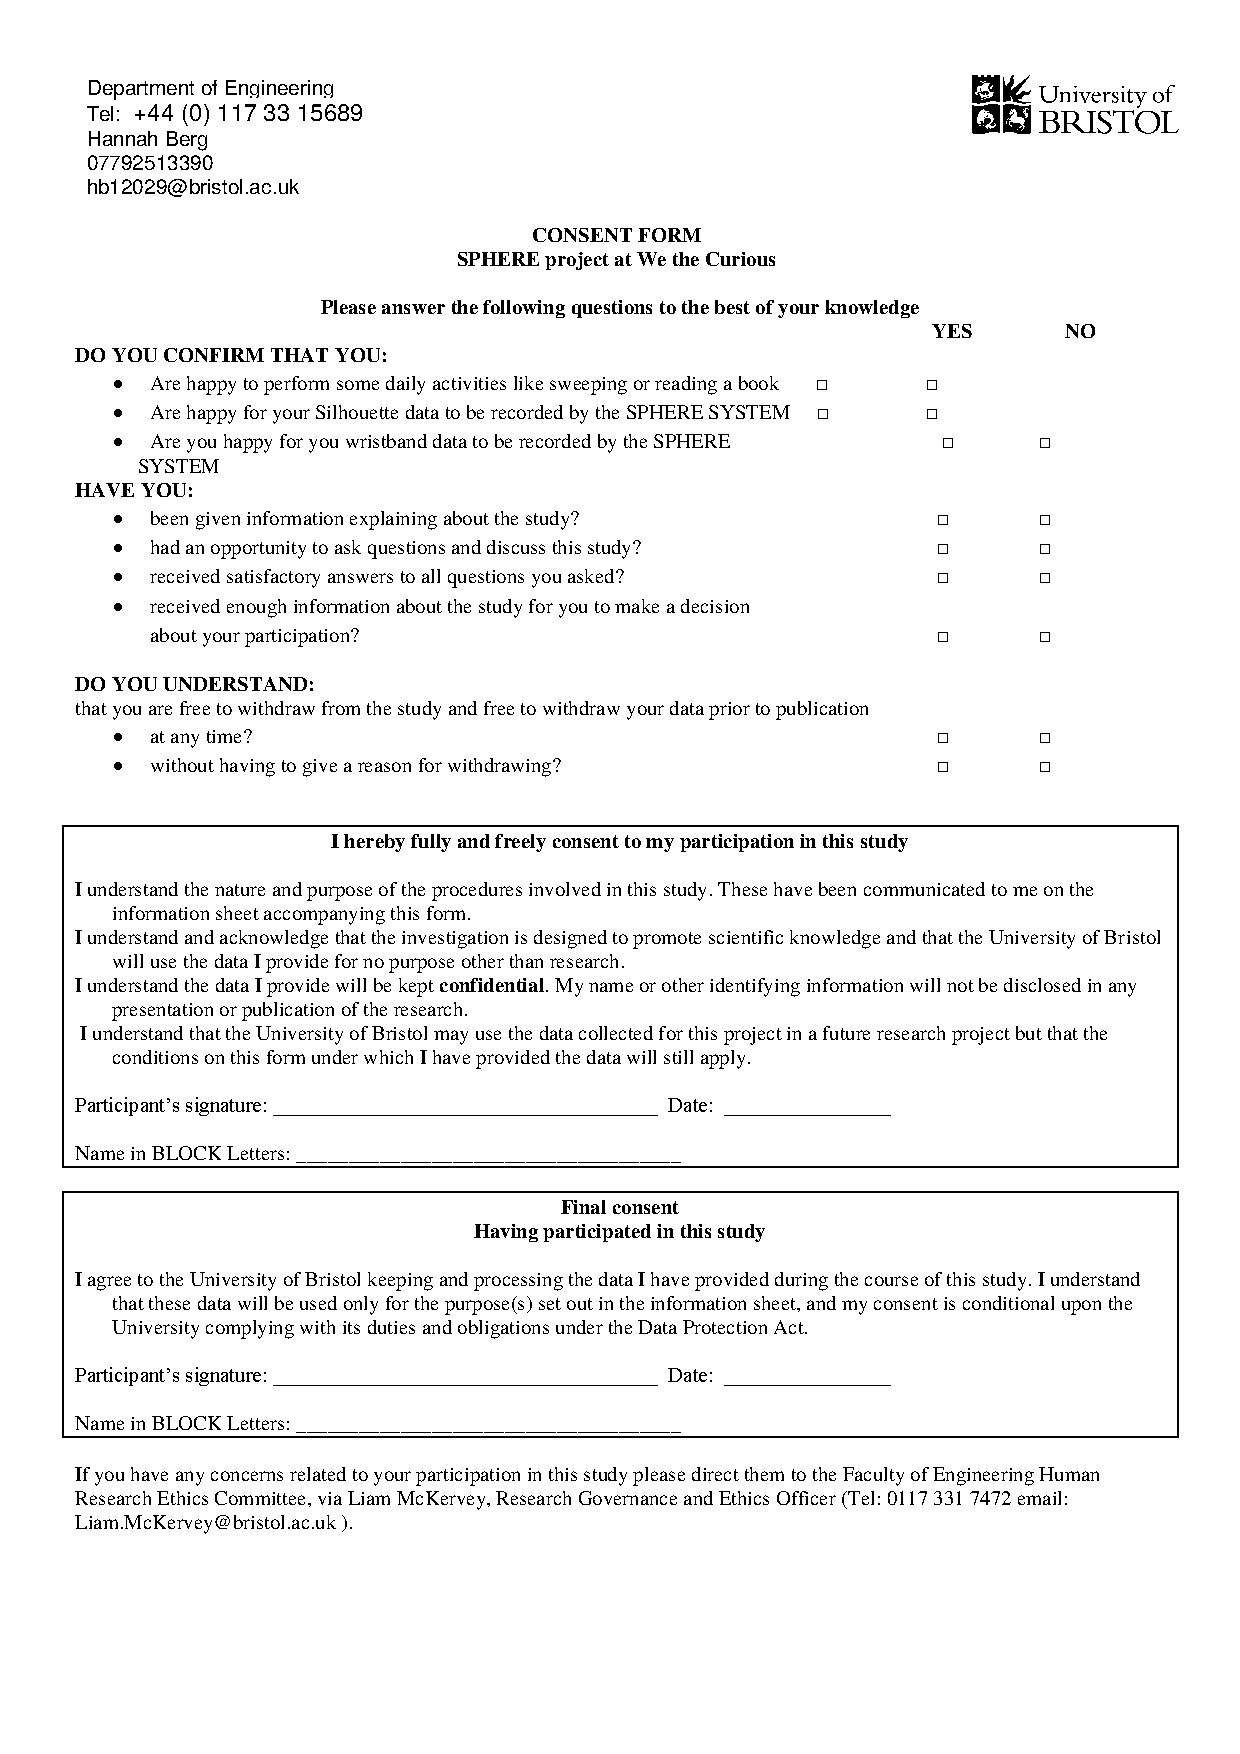
\includepdf[pages=-]{ethics/WeTheCurious_consent_form.pdf}

\newpage

\section{Appendix 2: sample Information sheets and Consent forms for research in
Special Education Needs Schools}

These samples were used for a study led by Dr. Nigel Newbutt, on VR with
autistic children. They formed a part of the ethics application successfully
submitted in 2018 by Dr. Newbutt to the UWE Ethics committee.

A similar process will be followed in the \project project, with full ethical
approval required before the start of each of the field studies.

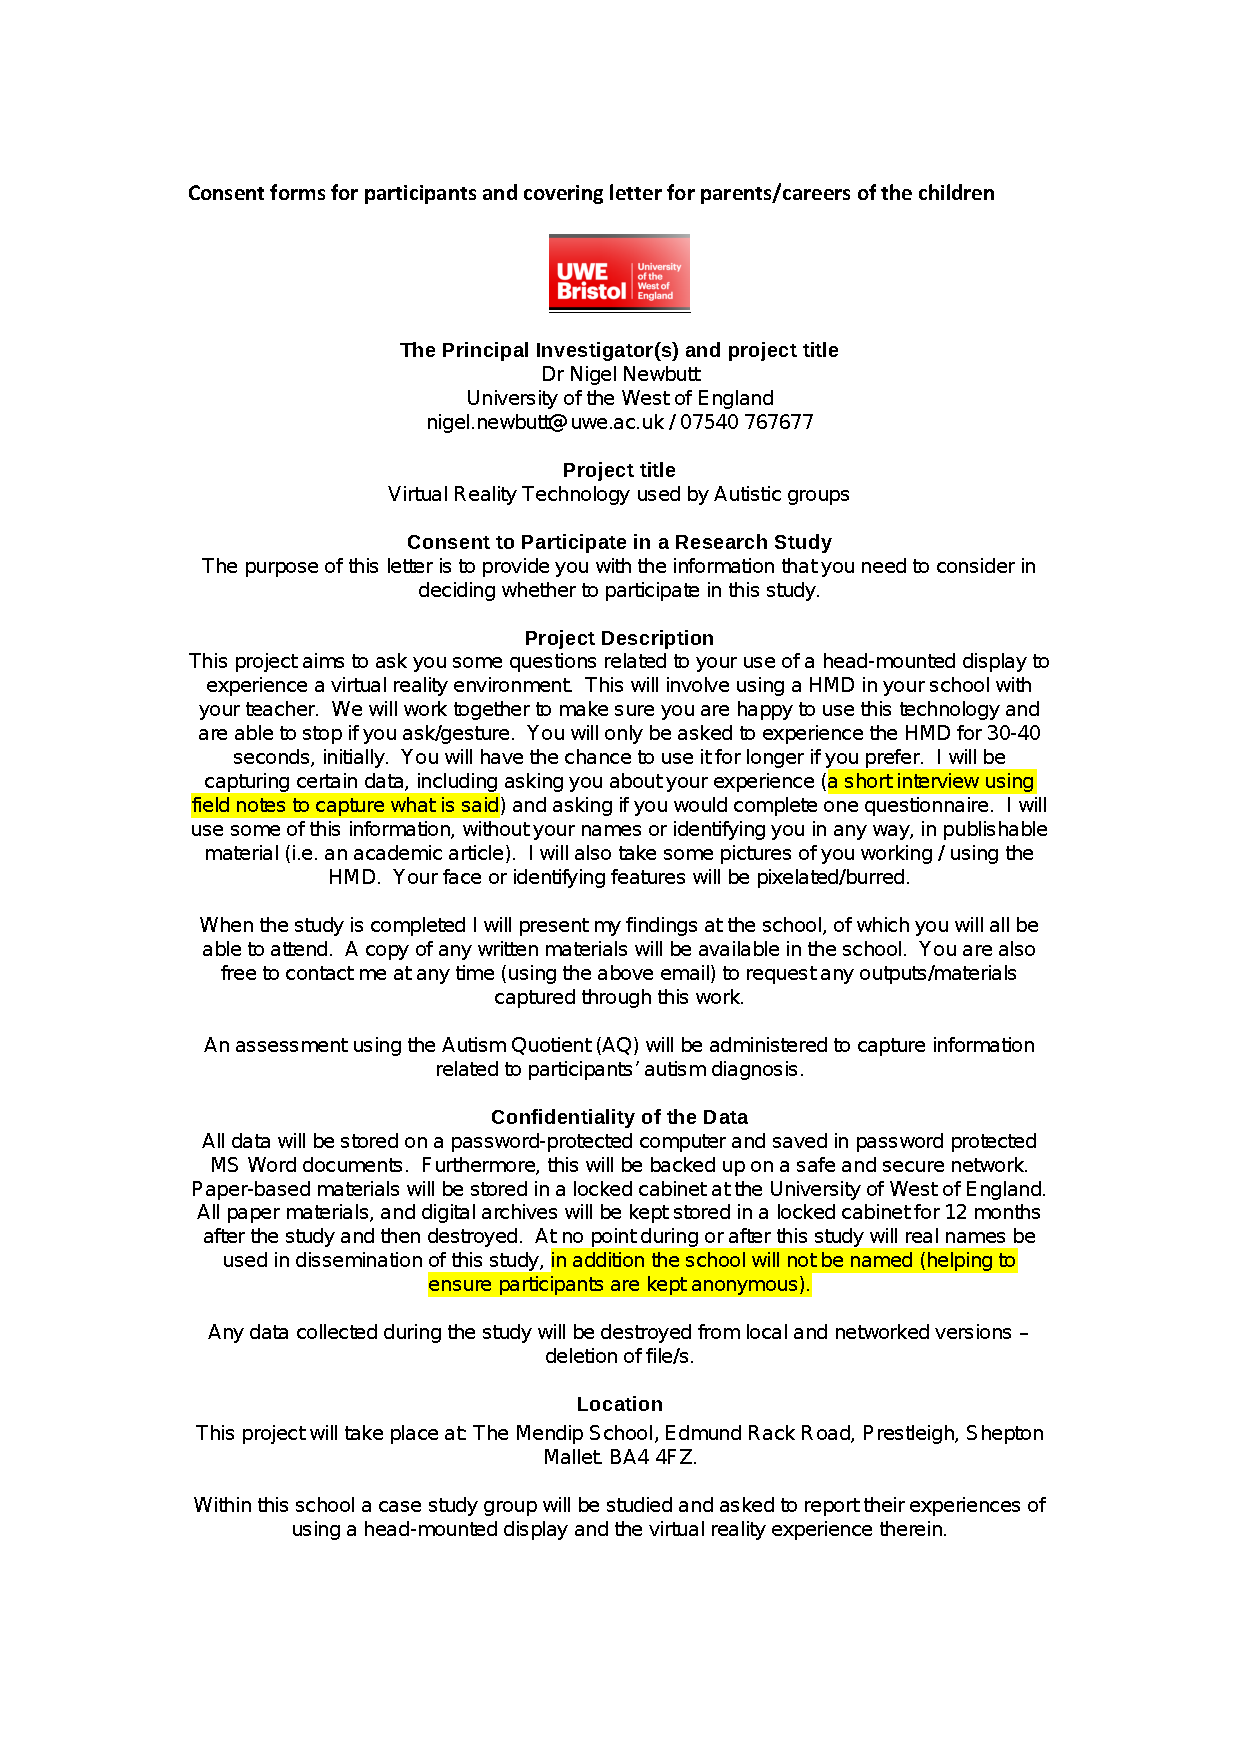
\includepdf[pages=-]{ethics/ethics-sample-nigel.pdf}

\end{document}

